% Gemini theme
% https://github.com/anishathalye/gemini

\documentclass[final,20pt]{beamer}

% ====================
% Packages
% ====================

\usepackage[ngerman]{babel}
\usepackage[T1]{fontenc}
\usepackage{lmodern}
\usepackage[size=a4,orientation=landscape,scale=1.6]{beamerposter}
\usetheme{gemini}
\usecolortheme{gemini}
\usepackage{graphicx}
\usepackage{tikz}
\usepackage{pgfplots}
\usepackage{svg}
\usepackage[font={large}]{caption}

% ====================
% Lengths
% ====================

% If you have N columns, choose \sepwidth and \colwidth such that
% (N+1)*\sepwidth + N*\colwidth = \paperwidth
\newlength{\sepwidth}
\newlength{\colwidth}
\setlength{\sepwidth}{0.02\paperwidth}
\setlength{\colwidth}{0.47\paperwidth}

\newcommand{\separatorcolumn}{\begin{column}{\sepwidth}\end{column}}
\addto\extrasngerman{\def\figureautorefname{Abb.}}

\addtobeamertemplate{headline}{} 
{\begin{tikzpicture}[remember picture, overlay]
	\node [anchor=north west, inner sep=0.3cm]  at (current page.north west)
	{
\includegraphics[height=2.5cm]{jufo}};
	\end{tikzpicture}
	\begin{tikzpicture}[remember picture, overlay]
	\node [anchor=north east, inner sep=0.3cm]  at (current page.north east)
	{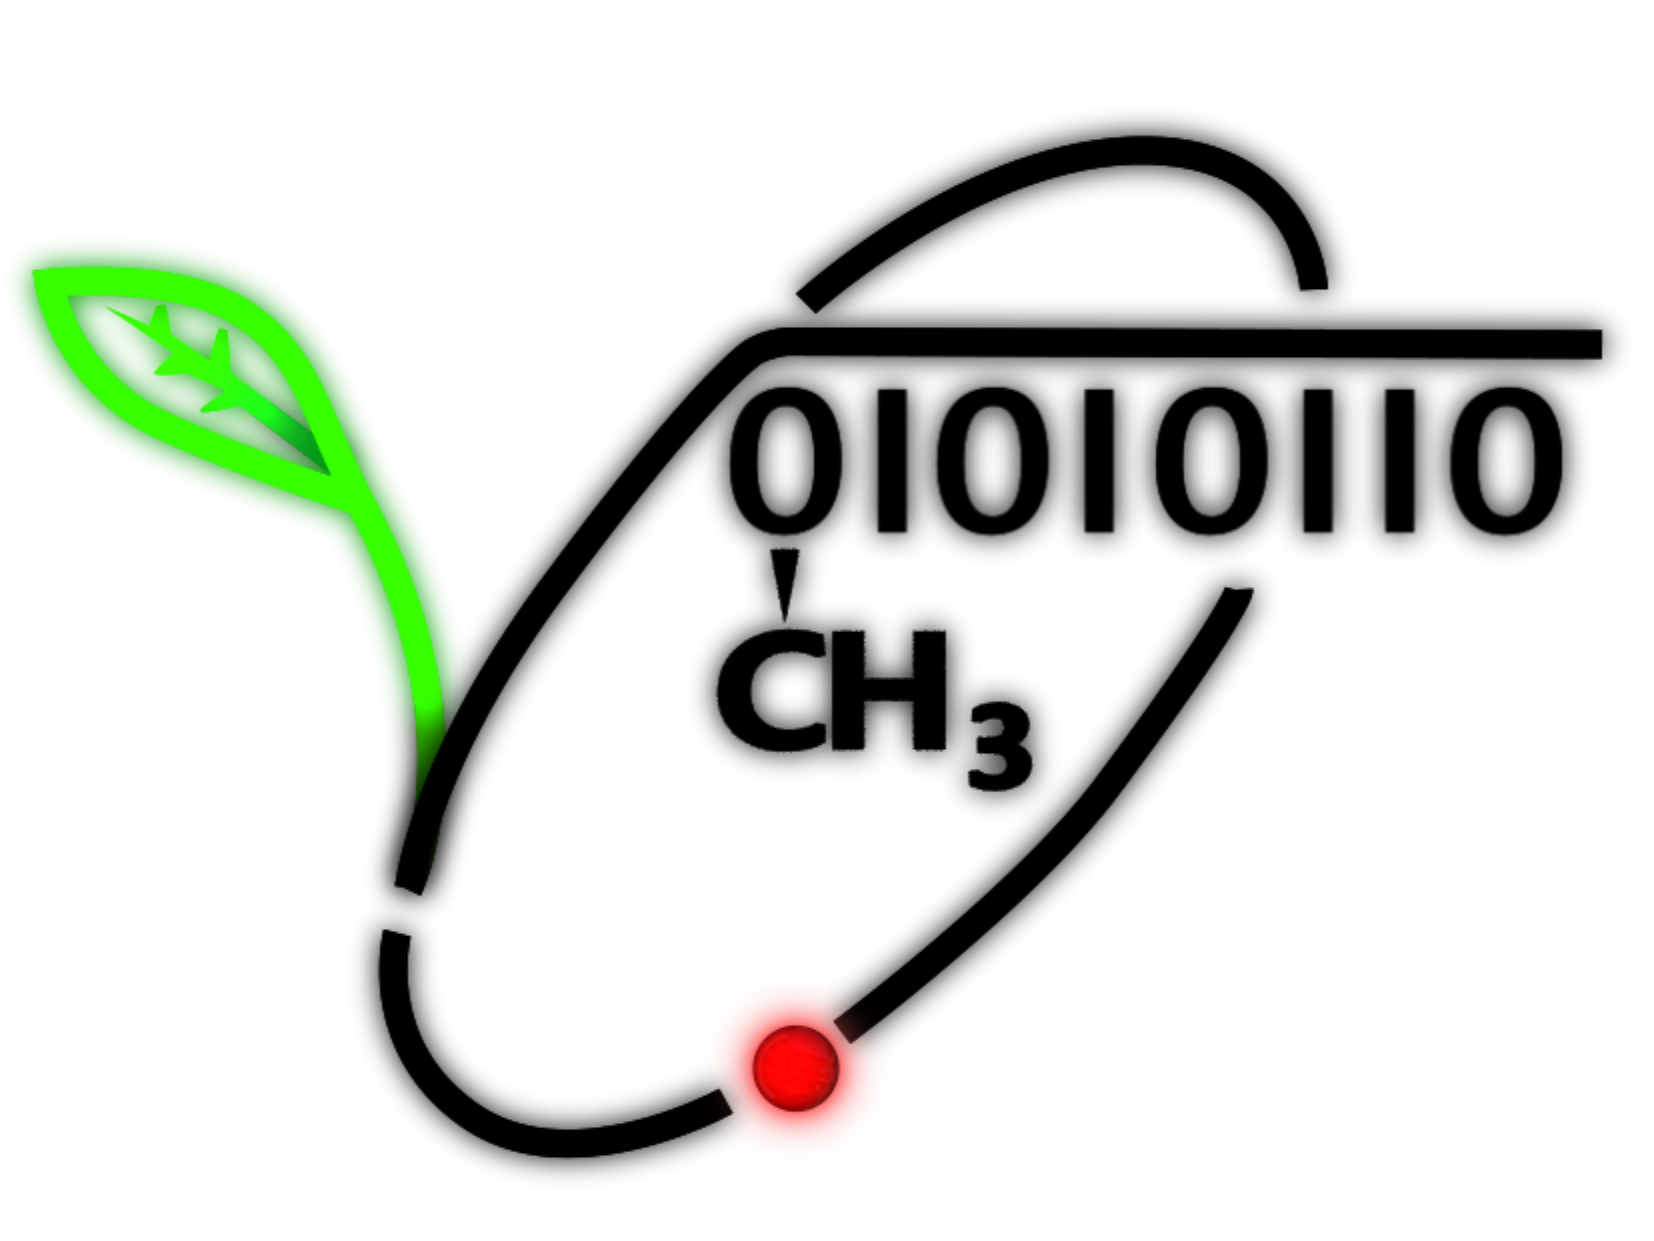
\includegraphics[height=2.5cm]{logo}};
	\end{tikzpicture}}
% ====================
% Title
% ====================

\title{Apoplexy - Ein Fitnesstracker zur Rehabilitation von Schlaganfall-Patienten}

%\author{Lukas Rost}
%\institute{Albert-Schweitzer-Gymnasium Erfurt}

% ====================
% Body
% ====================

\begin{document}

\begin{frame}[t]

\begin{columns}[t]
\separatorcolumn

\begin{column}{\colwidth}
   \begin{figure}
   	\centering 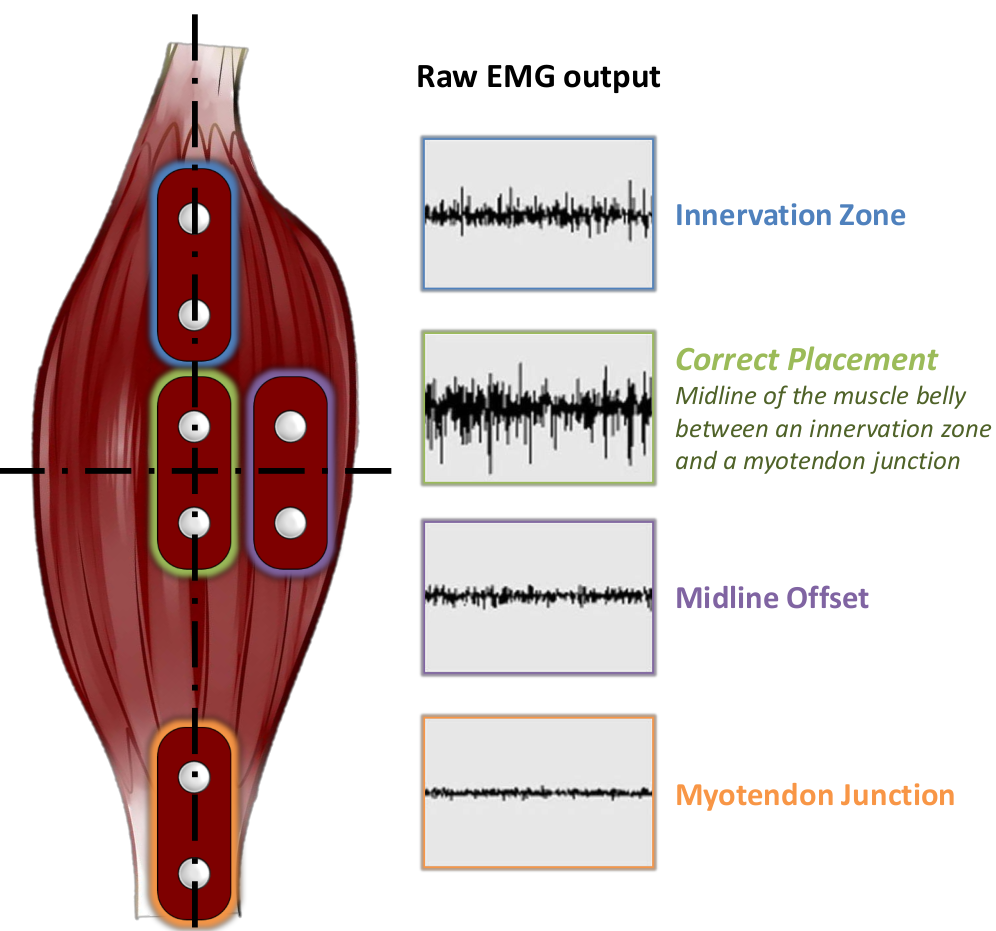
\includegraphics[width=\colwidth]{emg-output.png}
   	\caption{\centering Abhängigkeit des EMG-Signals von der Platzierung der Elektroden}
   \end{figure}
\end{column}

\separatorcolumn
\begin{column}{\colwidth}  
	
	\begin{figure}
		\centering 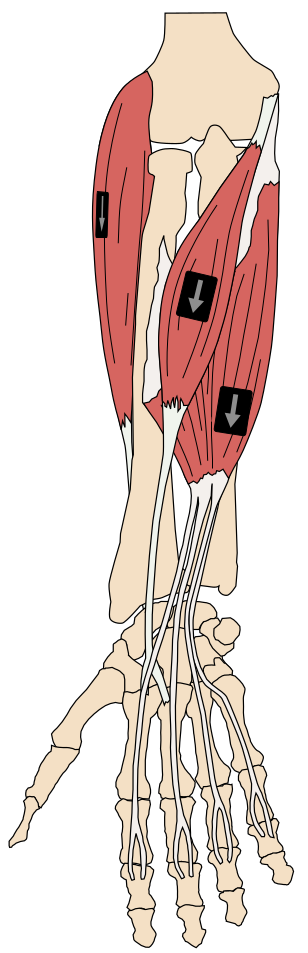
\includegraphics[scale=0.4]{unterarm-muskeln.png}
		\caption{\centering Muskeln des Unterarms}
	\end{figure}
\end{column}

\separatorcolumn
\end{columns}
\end{frame}

\end{document}